\chapter{API DE RECOMENDAÇÃO ORIENTADA À METADADOS}

Amparado pelos benefícios da utilização de mais de um método de recomendação, apresentando-os em forma de serviço, este capítulo detalha o funcionamento de uma \textbf{API REST como interface de recomendação}, fazendo uso de metadados provenientes do próprio usuário para criação, validação e interconexão entre as recomendações.

Como parte introdutória ao funcionamento, a seção \nameref{visao_geral} traça de forma abstrata as funcionalidades da API, apresentando os principais componentes e sua correlação. Posteriormente, nas seções \nameref{analisador}, \nameref{motor} e \nameref{interface}, tais funcionalidades são dissecadas de forma diminuir o nível de abstração. Por fim, os testes efetuados e as facilidades implementadas para a utilização da solução são abordados na seção \nameref{testes}.

\section{Visão Geral} \label{visao_geral}

A solução construída tem como função recomendar quaisquer itens a quaisquer usuários, sendo estes provenientes de uma fonte externa, fornecidos pelo usuário da API, nos padrões definidos pelos respectivos \textbf{metadados} existentes, também fornecidos inicialmente pelo usuário da API.

O usuário da API é definido como qualquer agente que tenha interações com a aplicação, humano ou programa, através requisições aos \textit{endpoints} fornecidos na documentação. Essas interações são acordadas pelo protocolo HTTP, usado como base em uma arquitetura REST \cite{rodriguez2008restful}. Dessa forma, o usuário da API pode utilizar qualquer interface que suporte o protocolo HTTP para desfrutar das funcionalidades da API, tornando-a multiplataforma e independente de bibliotecas de linguagens de programação específicas. As interações com os recursos da aplicação são efetuadas através dos seguintes métodos do protocolo HTTP:

\begin{itemize}
	\item \textbf{GET}: Interações que demandam a consulta de recursos.

	\item \textbf{POST}: Interações que demandam a criação de novos recursos.

	\item \textbf{PUT}: Interações que demandam a alteração de recursos existentes.

	\item \textbf{DELETE}: Interações que demandam a remoção ou desativação de recursos existentes.
\end{itemize}

Após o envio, a requisição é processada pela interface de usuário da API e, posteriormente, um retorno de sucesso ou erro finaliza a requisição. Para verificar o tipo do retorno da requisição, o usuário da API deve se ater aos \textit{status code} retornados pela API. Em caso de sucesso, por exemplo, a API retornaria um conteúdo JSON relacionado a requisição original e um \textit{status code} da faixa \textbf{2XX}. Já em caso de erro, a API retornaria um conteúdo de erro, anexo a um \textit{status code} da faixa \textbf{4XX} \cite{fielding1999hypertext}. Exemplos de requisição à API e o fluxo das mesmas após o envio podem ser visualizados nas figuras \ref{fetch_api}, \ref{postman} e \ref{interconnection}.

\begin{figure}[htp]
	\caption{\label{fetch_api}Exemplo de adição de item via \textit{fetch} API.}
	\begin{center}
		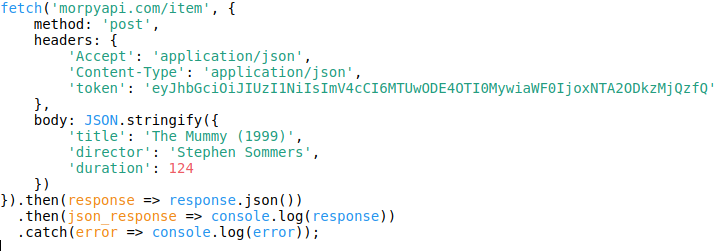
\includegraphics[scale=0.8]{images/fetch_api.png}
	\end{center}
	\hspace{5.5cm}{Fonte: O Autor.}
\end{figure}

\begin{figure}[htp]
	\caption{\label{postman}Exemplo de adição de item via Postman.}
	\begin{center}
		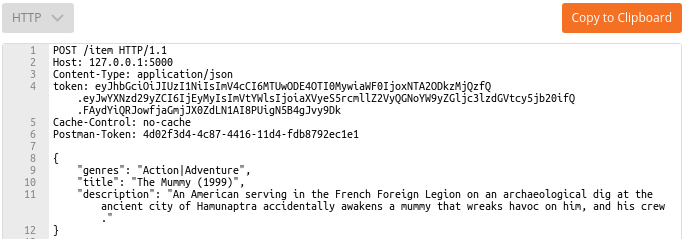
\includegraphics[scale=0.85]{images/postman.png}
	\end{center}
	\hspace{5.5cm}{Fonte: O Autor.}
\end{figure}

\begin{figure}[htp]
	\caption{\label{interconnection}Exemplo de fluxo de uma requisição à API.}
	\begin{center}
		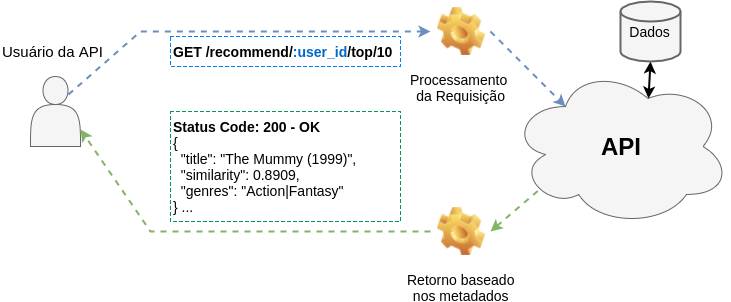
\includegraphics[scale=0.62]{images/interconnection.png}
	\end{center}
	\hspace{5.5cm}{Fonte: O Autor.}
\end{figure}

A figura \ref{interconnection} mostra um exemplo de requisição à API de recomendação. Nela, são requisitados os \textbf{dez} itens de maior similaridade a serem recomendados para o usuário denominado pelo parâmetro variável \textbf{\textit{user\_id}}. Este processo de requisição e resposta pode ser dividido em quatro partes principais:

\begin{enumerate}
	\item \textbf{Envio}: O usuário da API, devidamente autenticado, escolhe o \textit{endpoint} que corresponde as suas necessidades, enviando uma requisição através dos métodos HTTP previamente citados.

	\item \textbf{Interpretação}: A API receberá a requisição no devido \textit{endpoint}, interpretando-a e repassando-a através de chamadas internas das devidas funcionalidades.

	\item \textbf{Processamento}: Uma vez identificada a ação a ser executada, a API processa os dados (nesse caso as recomendações para o usuário \textbf{\textit{user\_id}}), posteriormente formatando-os em uma estrutura JSON.

	\item \textbf{Retorno personalizado}: Com a estrutura JSON processada em mãos, a API verifica os metadados atuais e retorna, com base nos atributos especificados como visíveis, uma estrutura JSON personalizada pelos desejo do usuário da API.
\end{enumerate}

Partindo da premissa que a solução deve atender modelos genéricos, serão fornecidos na inicialização da API os \textbf{metadados} de usuários, itens e avaliações, correspondendo a estrutura necessária pelo usuário da aplicação. Uma vez que os metadados sejam fornecidos, os dados relacionados devem respeitar as estruturas definidas. Tanto os usuários, itens e avaliações, quanto as futuras recomendações, serão persistidas em um banco de dados, a fim de centralizar as informações e diminuir o tempo de resposta das recomendações requisitadas.

De posse das estruturas de metadados fornecidas na inicialização, o usuário da solução poderá alimentar o sistema através das seguintes interfaces gerais:

\begin{itemize}
	\item \textbf{Metadados}: O usuário da API fornece a estrutura que irá compor cada um dos grupos abaixo. Essas estruturas definem os atributos de cada grupo, o tipo de cada atributo, a importância ou não do atributo nas recomendações, entre outras informações.

	\item \textbf{Usuários}: O usuário da API fornece os usuários aos quais deseja gerar algum tipo de recomendação. Esses dados serão utilizados posteriormente como referência aos itens e para definição da similaridade entre usuários.

	\item \textbf{Itens}: O usuário da API fornece os itens que serão recomendados aos usuários existentes. Os mesmos e seus atributos serão utilizados nas recomendações, atrelados a um usuário em questão.

	\item \textbf{Avaliações}: O usuário da API fornece as avaliações que ligam usuários a itens. Essas informações servem como união, apontando quais usuários estão relacionados a quais itens, sempre atrelando esta relação a uma avaliação numérica.
\end{itemize}

Tais ações de alimentação serão responsáveis por preencher os respectivos conjuntos anteriormente descritos e, a partir deles, construir os modelos de cada usuário e a matriz de avaliações, fundamentais para a geração das recomendações. Durante a requisição de uma recomendação, a solução definirá o método a ser utilizado e o mesmo fará as recomendações com base nos dados conhecidos, respeitando as propriedades descritas nos metadados. Um esquema do funcionamento geral da aplicação pode ser visto na \autoref{overview}.

\begin{figure}[h!tp]
	\caption{\label{overview}Visão geral da API.}
	\begin{center}
		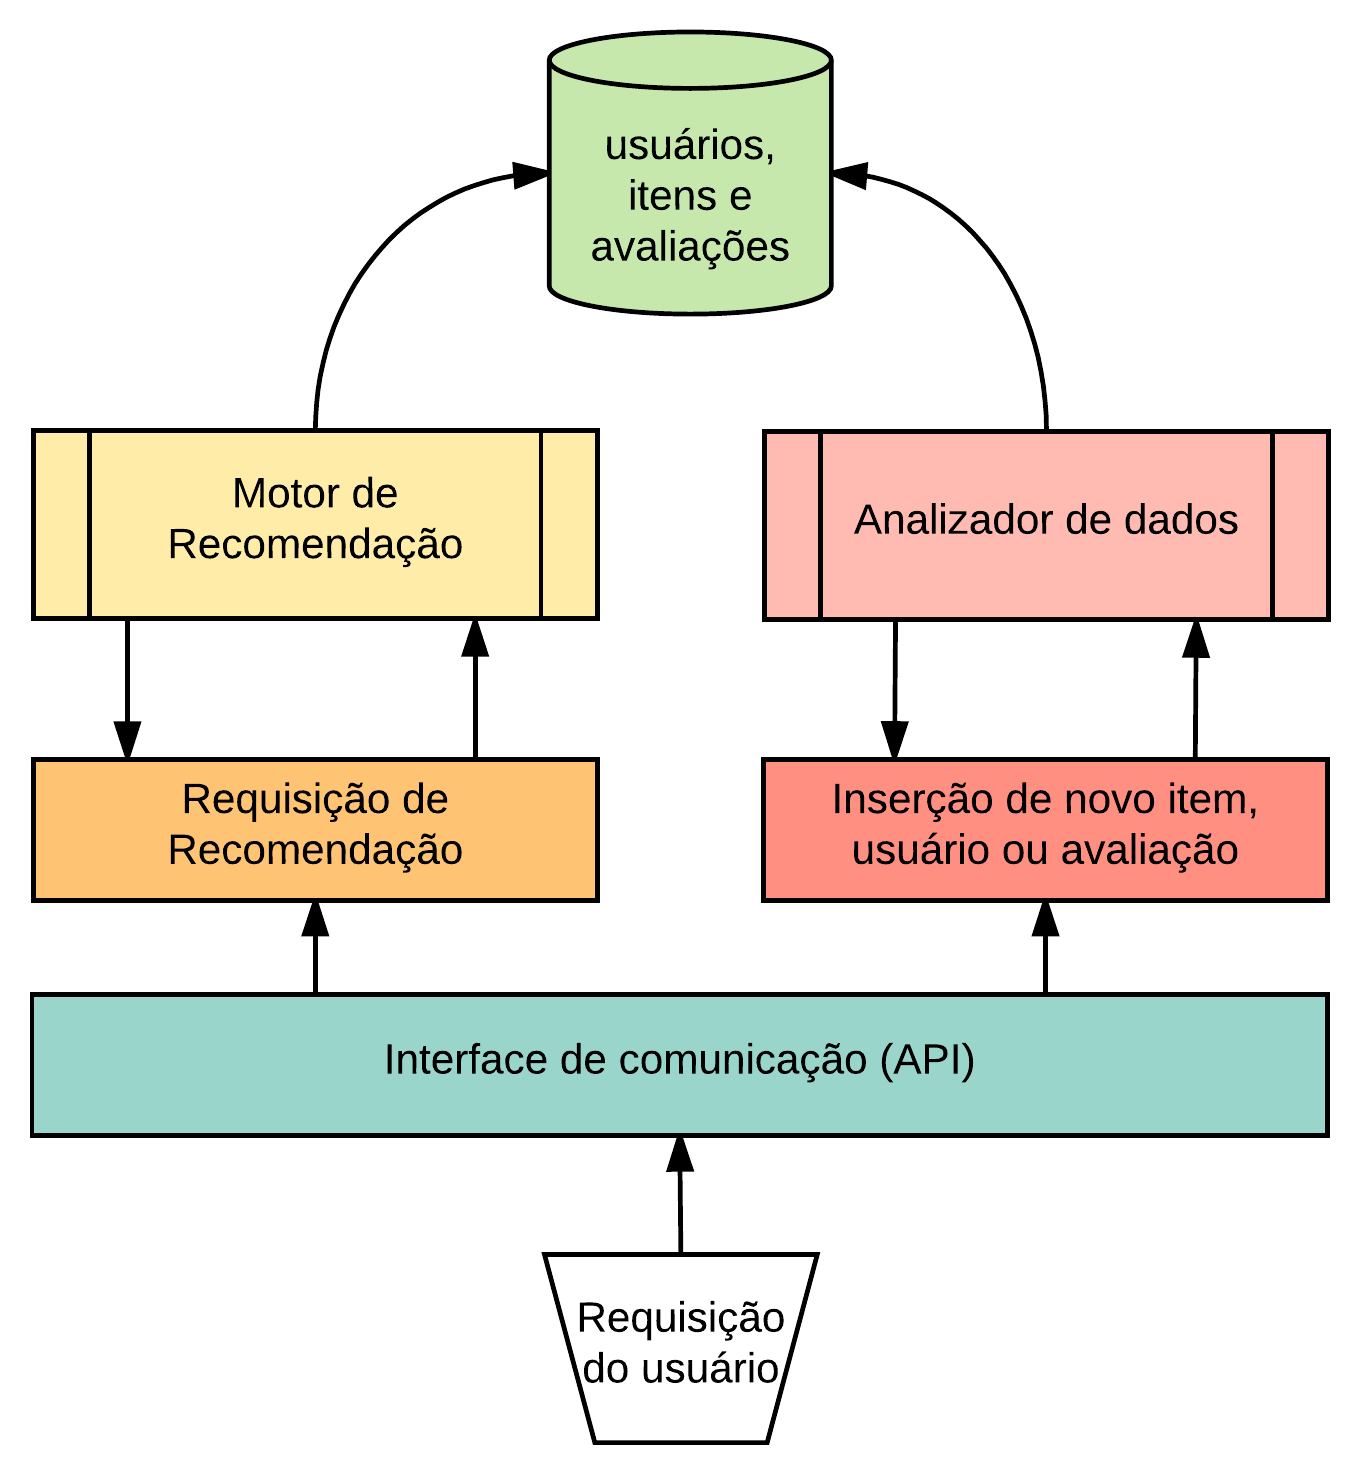
\includegraphics[scale=0.6]{images/MORPY_overview.png}
	\end{center}
	\hspace{5.5cm}{Fonte: O Autor.}
\end{figure}

De modo a complementar a visão da API apresentada pela figura \ref{interconnection}, a figura \ref{overview} apresenta o fluxo interno de funcionamento da API, apresentando uma distinção básica entre dois tipos de eventos: os eventos de \textbf{inserção ou atualização de dados} e os eventos de \textbf{geração e requisição de recomendações}. Ambos estão contidos no domínio de atuação da interface de comunicação com o usuário, a qual interpreta as requisições e processa as devidas respostas. Os módulos centrais correspondentes a estes domínios e suas interações podem ser subdivididas nos seguintes:

\begin{itemize}
	\item \textbf{Interface de Comunicação}: É o ponto de contato entre o cliente que utiliza a API e o domínio da aplicação, recebendo todas as requisições nos devidos \textit{endpoints}, processando-as e retornando os resultados. Este módulo é descrito detalhadamente na seção \nameref{interface}.

	\item \textbf{Analisador de Dados}: É o módulo responsável por contrastar as entradas da interface de comunicação com os metadados ativos. O trabalho do analisador de dados é validar o padrão de dados fornecido pelo cliente da API e persistir os dados corretos na base dados, notificando o motor de recomendação sobre quaisquer mudanças. Este módulo é descrito detalhadamente na seção \nameref{analisador}.

	\item \textbf{Motor de Recomendação}: É o módulo que definitivamente faz as recomendações. Ele se alimenta dos dados persistidos pelo analisador, gerando matrizes de relação, utilizadas para calcular o nível de similaridade entre usuário e itens, permitindo a persistência das recomendações na base de dados. Este módulo é descrito detalhadamente na seção \nameref{motor}.
\end{itemize}

Assim que uma requisição é recebida pela interface de comunicação, se a mesma for uma requisição de recomendação, a interface delega ao \textbf{motor de recomendações}, que busca as recomendações persistidas para o usuário em questão. Caso a requisição seja uma alteração de dados existentes, a interface delega ao \textbf{analisador de dados} a tarefa de validar, sempre baseando-se nos metadados atuais, os novos dados providos pelo usuário da API. Assim que esses dados são persistidos na base, o \textbf{motor de recomendações} identifica uma mudança na base e inicia um novo processo paralelo de treinamento para o dado modificado. Dessa forma, quando uma requisição for solicitada, basta o motor de recomendações consultar as recomendações já persistidas.

\section{A Interface de Comunicação} \label{interface}

Visando facilitar a comunicação com o usuário da API através do padrão REST, a interface de comunicação tem como principal função ser o ponto de contato entre o agente da requisição e as funcionalidades da API, atendendo a certos padrões de requisição e resposta que serão minuciosamente abordados nesta seção.

Ao passo que a API usa o padrão REST como base para a comunicação, é necessário que a mesma utilize um único padrão de dados para que ambos, usuário e API, tenham uma estrutura pré definida de possibilidades de envio e retorno. Dessa forma, o padrão de dados \textbf{JSON}, proposto por \citeonline{crockford2006application} foi o escolhido para servir como representação de dados da API, desde o recebimento de novos recursos (itens, usuários, etc.) até o retorno das recomendações. Um exemplo da representação JSON para as recomendações pode ser visto na figura \ref{json_example}.

\begin{figure}[h!tp]
	\caption{\label{json_example}Exemplo de estrutura JSON para recomendações.}
	\begin{center}
		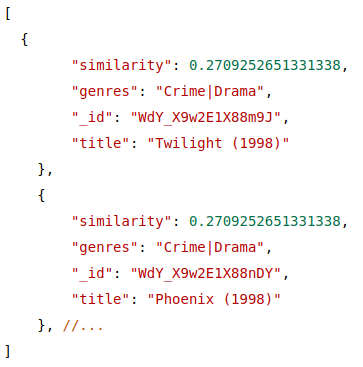
\includegraphics[scale=0.75]{images/json_example.png}
	\end{center}
	\hspace{5.5cm}{Fonte: O Autor.}
\end{figure}

Em outras palavras, esta seção apresenta o ponto de contato com a API, onde todas as requisições para modificações de recursos são feitas, visando melhorar a precisão das recomendações. Primeiro, é abordado o padrão de nomenclatura dos \textit{endpoints} na seção \ref{endpoints}, de modo a esclarecer de forma geral, toda a gama de possibilidade que o usuário da API tem ao utilizá-la. Em seguida, é apresentado o processo de autenticação na seção \ref{autenticacao}, necessário para que o usuário da API possa executar as requisições.

\subsection{Padrão de \textit{Endpoints}} \label{endpoints}

Toda a comunicação entre o agente das requisições e a API funciona através de \textit{endpoints} que modificam seus respectivos recursos. Recursos esses que são abstrações da base de dados, fazendo com que o agente das requisições possa interferir diretamente na evolução das recomendações, mesmo sem que haja uma interface gráfica. Um exemplo de recurso pode ser visualizado no quadro \ref{resource_example}.

\begin{quadro}[h!tp]

	\caption{\label{resource_example}Exemplo de recurso de \textit{endpoints} para o módulo item.}
	\begin{center}
	\begin{tabular}{|l|l|l|}
	\hline
	\textbf{Método HTTP} & \textit{\textbf{Endpoint}} & \textbf{Descrição}          \\ \hline
	POST                 & /item                      & Cria um novo item           \\ \hline
	GET                  & /item/:item\_id 			  & Retorna um item específico  \\ \hline
	PUT                  & /item/:item\_id            & Altera um item específico   \\ \hline
	DELETE               & /item/:item\_id            & Deleta um item específico   \\ \hline
	GET                  & /item                      & Retorna todos os itens      \\ \hline
	\end{tabular}
	\end{center}

	\hspace{2.5cm} {\fontsize{10pt}{\baselineskip}\selectfont Fonte: O autor.}
\end{quadro}

Analisando o quadro \ref{resource_example}, nota-se que um mesmo \textit{endpoint} pode apontar para diferentes funções, uma vez que o método HTTP que encabeça a requisição também é levado em consideração. Além disso, é importante ressaltar que cada par de \textbf{método HTTP} e \textbf{\textit{endpoint}} correspondem diretamente a um \textbf{controlador} da API, que recebe os parâmetros variáveis da requisição (no quadro \ref{resource_example} representando por \textit{item\_id}) e os repassa aos serviços. Sendo assim, os controladores poderiam ser definidos como as "portas de entrada" da API, direcionando a execução de cada funcionalidade.

Para aumentar o nível de abstração do funcionamento da API, o padrão de \textit{endpoints} utiliza do atributo de identificador único de cada módulo, previamente definido nos metadados de itens, usuários e avaliações, para o acesso a um recurso específico. Dessa forma, o usuário da API pode utilizar os seus próprios identificadores de sua base de dados externa, para acessar os mesmos recursos na base interna da aplicação. O modo de declaração deste atributo e seu tipo de dado esperado podem ser vistos na seção \nameref{analisador:padrao_metadados}. 

\subsection{Autenticação} \label{autenticacao}

Como forma de aumentar a segurança durante as requisições e, principalmente, garantir que apenas os usuários com acesso ao serviço façam requisições, a API conta com um sistema de autenticação via \textit{token}.

Antes da primeira inicialização, o \textit{script} gera um \textit{token} único para o usuário da API, que será posteriormente concatenado com uma palavra secreta nos arquivos de configuração, além da data e hora atuais da requisição de autenticação. O resultado final é um \textit{token} temporário, com validade de até quinze dias, que será utilizado, obrigatoriamente, no cabeçalho de quaisquer requisições aos recursos da API.

Do mesmo modo que o agente das requisições precisa incluir o \textit{token} temporário no cabeçalho das requisições, a API precisa verificar a validade deste \textit{token}. Para que isso seja possível, foi criada uma classe intermediária (\textit{middleware}) que intercepta todas as requisições, exceto a requisição de autenticação. Essa classe, por sua vez, verifica a existência do \textit{token} no cabeçalho da requisição bem como sua validade. Caso o \textit{token} não exista ou não remeta a um usuário de API válido, o \textit{middleware} bloqueia a execução da requisição, retornando uma mensagem de erro e um \textit{status code} igual a \textbf{403} - "\textit{Forbidden}". Um exemplo requisição de autenticação pode ser visto na figura \ref{auth_example}.

\begin{figure}[h!tp]
	\caption{\label{auth_example}Exemplo de autenticação.}
	\begin{center}
		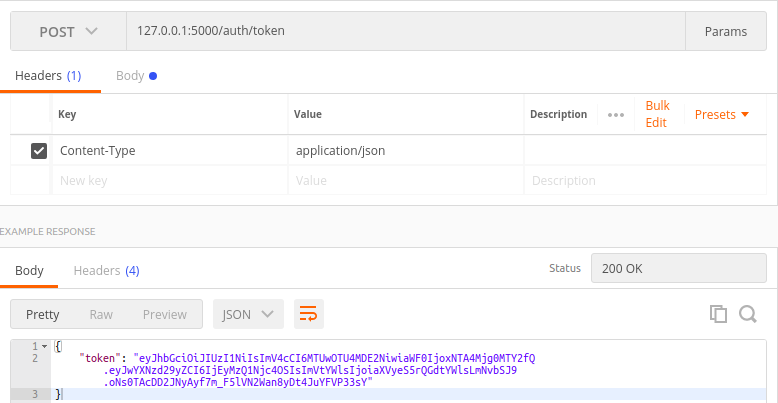
\includegraphics[scale=0.6]{images/auth_example.png}
	\end{center}
	\hspace{5.5cm}{Fonte: O Autor.}
\end{figure}

\section{O Analisador de Dados} \label{analisador}

Para tornar possível a geração de recomendações de forma genérica, através dos metadados, foi necessária a construção de um módulo dedicado exclusivamente a este fator. O \textbf{analisador de dados} tem como principal objetivo cruzar as novas informações, repassadas pela interface de comunicação, com os metadados correntes.

Por exemplo, para que um novo item seja adicionado ao conjunto de itens conhecidos e, posteriormente, treinado contra os outros itens, é necessário que o analisador de dados verifique se todos os atributos relevantes para as recomendações estão preenchidos, se os tipos dos campos fornecidos condizem com os tipos especificados nos metadados, etc.

Em síntese, esta seção apresentará os principais componentes do analisador de dados. Primeiro apresentando os padrões utilizados para a orientação a metadados na seção \ref{analisador:padrao_metadados}, em seguida, os modelos gerados pelos metadados e sua utilização em toda a aplicação, aprofundados na seção \ref{analisador:modelos} e, por fim, como é feita a persistência destes dados na seção \ref{analisador:persistencia}.

\subsection{Padrão de Metadados} \label{analisador:padrao_metadados}

Uma vez que não se sabe qual o padrão de JSON a se retornar ao usuário, ou quais os campos relevantes para a geração das recomendações, ou ainda quais sequer são os nomes dos atributos, os metadados são as estruturas, previamente definidas e passíveis de personalização, fornecidas pelo usuário na inicialização da aplicação. Estas estruturas são enviadas através de uma estrutura JSON para os \textit{endpoints} respectivos, divididos em três categorias:

\begin{itemize}
	\item \textbf{Usuários}: Definem os nomes dos atributos, obrigatórios ou não, que compõem o modelo de usuário, os tipos de cada atributo, a quantidade máxima de caracteres, se é recomendável ou não e seu peso. Além disso os metadados de usuários apontam o identificador único do usuário.

	\item \textbf{Itens}: Assim como os usuários, definem os nomes de cada atributo, obrigatórios ou não, do item e suas demais características. Além disso, é definida a exibição de cada atributo do item no retorno das recomendações e seu identificador único.

	\item \textbf{Avaliações}: Definem obrigatoriamente o campo de identificador único do usuário e o campo de identificador único do item, amarrando efetivamente as duas entidades. Além disso, definem o tipo de avaliação que será empregada (binária ou não).
\end{itemize}

Para ilustrar o processo de definição dos metadados, a figura \ref{metadata} mostra um exemplo real dos metadados inciais para o modelo de \textbf{item}. Estes atributos podem ser modificados posteriormente através do mesmo \textit{endpoint} utilizando o método PUT do HTTP. Caso o qualquer atributo sofra posterior alteração, os metadados são salvos com o status \textbf{"\textit{active:false}"}, orientado que o mesmo não é mais válido. Em seguida, um novo conjunto de metadados é criado com o atributo \textbf{"\textit{active:true}"} e as modificações solicitadas pelo usuário.

\begin{figure}[htp]
	\caption{\label{metadata}Exemplo de declaração de metadados para o item.}
	\begin{center}
		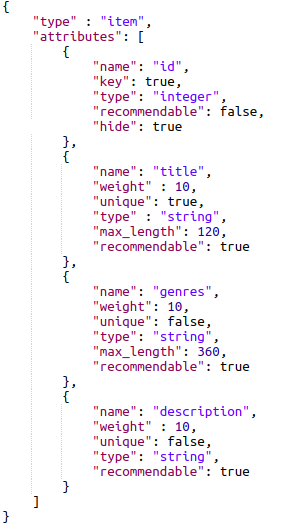
\includegraphics[scale=0.8]{images/metadata.png}
	\end{center}
	\hspace{5.5cm}{Fonte: O Autor.}
\end{figure}

Analisando a figura \ref{metadata} nota-se um conjunto de chaves pré-definidas para a estrutura declarada. A razão dessas chaves possuírem suas definições \textbf{obrigatórias e pré-definidas} é o fato de que as mesmas moldam todas as outros atributos dinamicamente atribuídos aos modelos de itens, usuários e avaliações, consequentemente moldando o banco de dados. Sendo assim, cada chave da estrutura definida na figura é utilizada como atributo chave para alguma decisão estrutural dentro da API. As chaves definidas na figura possuem as seguintes funcionalidades:

\begin{itemize}
	\item \textbf{\textit{type}}: Fora da chave \textbf{\textit{"attributes"}}, define o tipo do grupo de metadados que correspondem os atributos declarados. Dentro de um atributo, define o tipo do dado ao qual o atributo espera um valor, podendo ser qualquer tipo natural: \textbf{\textit{string}}, \textbf{\textit{integer}}, \textbf{\textit{float}}, etc. Espera um valor do tipo \textbf{\textit{string}}.

	\item \textbf{\textit{attributes}}: Declara a lista de atributos pertencentes ao \textit{type}, neste caso ao item.  Espera um valor do tipo \textbf{\textit{array}}.

	\item \textbf{\textit{name}}: Define o nome de um atributo, o qual será utilizado como chave do atributo no banco de dados e na construção dinâmica do modelo. Espera um valor do tipo \textbf{\textit{string}}.

	\item \textbf{\textit{key}}: Define se o atributo é ou não um identificador único. Será utilizado posteriormente para ligar os usuários a itens e para fazer as consultas dos endpoints.  Espera um valor do tipo \textbf{\textit{boolean}}.

	\item \textbf{\textit{hide}}: Define se o atributo será ou não exibido no JSON de retorno. Espera um valor do tipo \textbf{\textit{boolean}}.

	\item \textbf{\textit{unique}}: Define se o atributo deve ser único na base de dados ou não. Caso o seu valor seja verdadeiro (\textit{true}), o analisador de dados retornará um erro para a requisição, caso este atributo já exista. Espera um valor do tipo \textbf{\textit{boolean}}.

	\item \textbf{\textit{nullable}}: Por padrão, todos os atributos declarados nos metadados serão obrigatórios na inserção de novos registros. Caso este atributo estiver com o valor verdadeiro (\textit{true}), o mesmo torna-se opcional. Espera um valor do tipo \textbf{\textit{boolean}}.

	\item \textbf{\textit{max\_length}}: Declara a quantidade máxima de tamanho/caracteres que o campo suporta. Será utilizada posteriormente para barrar entradas maiores que esse valor no banco de dados. Espera um valor do tipo \textbf{\textit{integer}}.

	\item \textbf{\textit{recommendable}}: Define se o atributo será utilizado como base para as recomendações ou não. Será utilizado pelo motor de recomendações para levar em consideração apenas os atributos que o usuário da API julgar relevantes. Espera um valor do tipo \textbf{\textit{boolean}}.

	\item \textbf{\textit{weight}}: Se o atributo \textbf{\textit{recommendable}} for verdadeiro (\textit{true}), define o peso do atributo nos cálculos de recomendação. O peso varia de um a dez. Espera um valor do tipo \textbf{\textit{integer}}.
\end{itemize}

Assim que a API toma conhecimento dos metadados, já é possível ao usuário da API preencher o banco de dados com seus usuários, itens e avaliações iniciais.

Por outro lado, a API, antes de persistir os metadados na base, adiciona alguns atributos para facilitar o gerenciamento posterior, dentre eles: um atributo de \textbf{data} para representar a data de inserção, um atributo de \textbf{versão} para identificar a evolução da estrutura e, por fim, um atributo \textbf{\textit{active}} que, se possuir valor verdadeiro, determina qual o grupo de metadados que está atualmente em vigor. Uma linha do tempo dos metadados com as modificações feitas pelo usuário da API pode ser acessada através do endpoint \textbf{/metadata/:metadata\_type/history}.

\subsection{Modelos de Metadados, Itens, Usuários e Avaliações} \label{analisador:modelos}

Para gerenciar o fluxo de dados dentro da API, se fez necessária a criação de modelos encapsuladores, que tem como função abstrair a complexidade da validação, gerenciamento e representação destes dados dinâmicos.

Levando em conta que não se sabe quais serão os atributos de um item, por exemplo, antes do tempo de execução, é necessário que a validação seja feita com base não nos atributos do item, mas sim nos atributos previamente definidos pelos metadados do mesmo. Dessa forma, é possível contrastar o padrão esperado, definido nos metadados, com os dados efetivamente enviados pelo usuário da API.

Levando em consideração os atributos do grupo de metadados apresentados na seção \nameref{analisador:padrao_metadados}, a figura \ref{validation} apresenta um exemplo de validação, feito na linguagem Python, utilizando tais atributos para dinamicamente verificar o padrão do item recebido através de uma requisição do usuário da API. As partes irrelevantes do código foram omitidas para melhor apresentação.

\begin{figure}[h!tp]
	\caption{\label{validation}Validação baseada nos metadados.}
	\begin{center}
		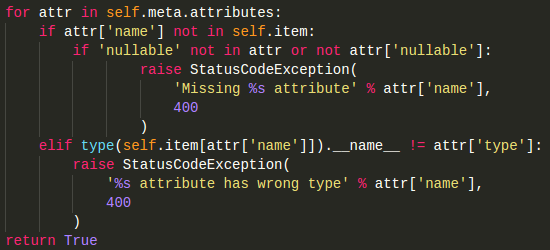
\includegraphics[scale=0.83]{images/python_validation.png}
	\end{center}
	\hspace{5.5cm}{Fonte: O Autor.}
\end{figure}

Ao contrário das aplicações comuns, que delegam o trabalho de manter a saúde dos dados para a base de dados, esta estratégia não é viável nesta aplicação devido ao fato da estrutura do banco de dados não só ser dinâmica, como também totalmente customizada pelo usuário da API.

Dessa forma, o trecho de código mostrado na figura \ref{validation}, em conjunto outras classes auxiliares, tem como objetivo garantir que, apenas os dados enviados dentro do padrão descrito no grupo de metadados correspondente, serão persistidos no banco de dados.

Sendo assim, a lógica da figura pode ser descrita da seguinte forma: primeiro a aplicação percorre todos os atributos dos metadados correspondente. Para cada atributo descrito nos metadados, a aplicação testa se este atributo, caso seja obrigatório (\textbf{\textit{nullable:false}}), está contido no JSON recebido pelo \textit{endpoint}. Se o atributo obrigatório não existir, a aplicação retorna um JSON de erro com o \textit{status code} igual a \textbf{400}, indicando uma \textbf{\textit{bad request}}. Caso o atributo exista, a aplicação testa se o tipo do dado recebido condiz com o tipo declarado nos metadados (\textbf{\textit{type}}). Uma vez que todos os atributos obrigatórios são satisfeitos pelo JSON recebido, a aplicação o persiste na base de dados.

Para ilustrar o processo, a figura \ref{validation_schema} demonstra um exemplo do fluxo interno do \textbf{analisador de dados}, desde o recebimento da informação, até a persistência e posterior retorno da mesma. O código completo dos modelos de dados pode ser visto no apêndice \nameref{source_code}.

\begin{figure}[h!tp]
	\caption{\label{validation_schema}Esquema do fluxo do analisador de dados.}
	\begin{center}
		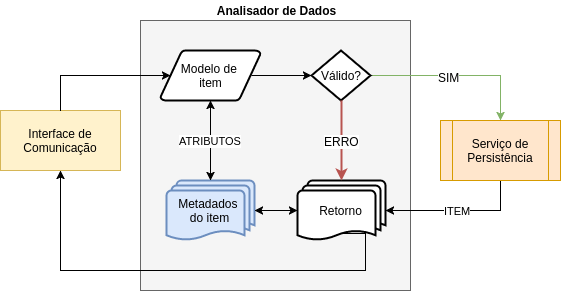
\includegraphics[scale=0.8]{images/validation.png}
	\end{center}
	\hspace{5.5cm}{Fonte: O Autor.}
\end{figure}

Representando o fluxo de modificação dos dados de um item específico, nota-se na figura \ref{validation_schema}, que o analisador de dados recebe as devidas requisições através da interface de comunicação, transformando-as em modelos dos recursos. Assim que os modelos são construídos, são carregados da base de dados os metadados vigentes, utilizados posteriormente no contraste e validação destes modelos. Caso o modelo de item, representação abstrata da requisição do usuário da API, seja válido, o mesmo é persistido na base de dados e, posteriormente, enviado como retorno. Caso o item não seja válido, ao invés de persisti-lo na base, uma mensagem de erro é enviada como retorno ao usuário da API.

Todavia, em caso de sucesso na persistência, antes de efetivamente retornar o \textit{feedback} ao agente da requisição, o analisador de dados constrói a estrutura de retorno a partir dos atributos dos metadados em vigor. O atributo declarado como identificador único (\textbf{\textit{key:true}}) nos metadados é obrigatoriamente adicionado na estrutura de retorno, uma vez que é utilizado como parâmetro base em todos os \textit{endpoints} relacionados. Além disso, o atributo \textbf{\textit{hide}} define se o atributo existente será exibido ou não no JSON de retorno.

\subsection{Persistência} \label{analisador:persistencia}

A base de um sistema de recomendação é o conhecimento prévio, uma vez que, independente da métrica ou método utilizados, todos utilizam do cruzamento de informações conhecidas para gerar predições (vide seção \ref{recommender_systems}). Dessa forma, é necessário que alguma estratégia eficiente de armazenamento e consulta seja utilizada, tendo em vista que o cruzamento dessas informações pode gerar matrizes excedendo milhões de linhas e colunas \cite{gomez2016netflix}.

Visando utilizar uma estratégia de persistência que se destacasse no processamento de grandes conjuntos de dados, ponto essencial para boas recomendações, a API implementa uma persistência utilizando um banco de dados não relacional (NoSQL) orientado a documentos \cite{leavitt2010will}, que além de proficiente no manejo dos dados, também persiste os mesmos em estruturas baseadas em JSON, como apresentado por \citeonline{padhy2011rdbms}.

Devido ao JSON ser o padrão escolhido para a estrutura de dados da aplicação, a similaridade entre o documento armazenado no banco de dados e o JSON de retorno ao usuário da API é muito pequena, reduzindo o nível de complexidade como um todo. Além disso, é permitida a inserção de documentos dinâmicos, sem um padrão previamente definidos em tabelas e campos, sendo possível inserir novos atributos em itens, usuários e avaliações apenas declarando-os nos metadados, sem a necessidade de modificar a estrutura da base de dados.

A fim de abstrair este processo para os outras partes da aplicação, foram criadas serviços de persitência para cada módulo existente, responsáveis por administrar toda a comunicação com o banco de dados. Tais serviços são utilizados tanto pelo \textbf{analisador de dados} quando pelo \textbf{motor de recomendações}, seja para a persistência de novas recomendações recém geradas ou para novos itens enviados pelo usuário da API através da interface de comunicação. A figura \ref{persistence} demonstra o processo de construção dinâmica do item através do modelo e sua persistência no banco de dados.

\begin{figure}[h!tp]
	\caption{\label{persistence}Esquema do serviço de persistência.}
	\begin{center}
		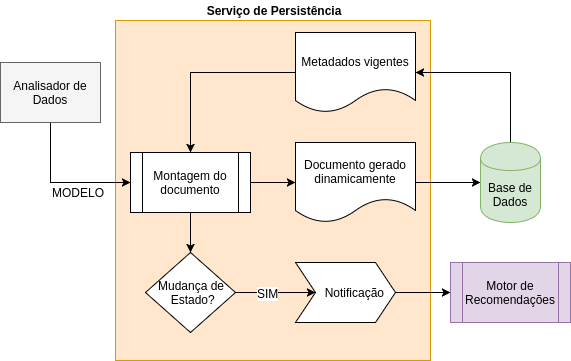
\includegraphics[scale=0.83]{images/persistence.png}
	\end{center}
	\hspace{5.5cm}{Fonte: O Autor.}
\end{figure}

Como apresentado na figura \ref{persistence}, o serviço de persistência recebe um modelo, previamente criado e validado pelo \textbf{analisador de dados}. Este modelo será contrastado com os metadados vigentes para geração dinâmica de um documento no formato necessário para sua inserção no banco de dados. Assim como nos \textit{endpoints} da interface de comunicação, os serviços de persitência usam como parâmetros para administração de documentos específicos o identificador único (\textbf{\textit{key:true}}) declarado nos metadados, gerando documentos com base neste identificador.

Além da persistência do modeo recebido, o serviço de persistência também é encarregado de notificar o motor de recomendações de quaisquer modificações ou adições aos documentos existentes. Esta notificação é necessária para que o motor de recomendações saiba quando é necessário treinar novos documentos recém adicionados, ou quando treinar novamente documentos que mudaram seu estado. O processo de recebimento das notificações e treinamento da base pode ser visto na seção \nameref{motor}.

\section{O Motor de Recomendações} \label{motor}

Toda a estrutura acima descrita tem como objetivo possibilitar o funcionamento do motor de recomendações, fornecendo os dados necessários para a geração das matrizes de predição. O motor de recomendações, por sua vez, tem como objetivo efetivamente gerar as recomendações para quaisquer usuários ou itens, levando em consideração o padrão de gostos do usuário, o conteúdo do item e a relação entre ambos.

Do mesmo modo que o analisador de dados, o motor de recomendações faz uso dos modelos de usuários, itens e avaliações visando obter informações geradas dinamicamente com o uso dos metadados. Dentre as informações relevantes para o motor de recomendações estão:

\begin{itemize}
	\item \textbf{Atributos recomendáveis}: Os atributos marcados com a \textit{tag} \textbf{\textit{recommendable:true}} mapeam quais atributos devem ser levados em consideração pelos algoritmos.

	\item \textbf{Peso dos atributos}: Os atributos marcados com a \textit{tag} \textbf{\textit{weight}} mapeam quais atributos, além de recomendáveis, recebem um peso diferenciado para os algoritmos, maximizando o nível de personalização.

	\item \textbf{Identificadores únicos}: Os atributos marcados com a \textit{tag} \textbf{\textit{key:true}} identificam quais informações serão utilizadas como identificadores de itens e usuários durante a execução dos algoritmos, permitindo sua correta persistência, além de manter a integridade das recomendações. Além disso, permitem identificar quais usuários avaliaram quais itens, informação essencial para a recomendação colaborativa.

	\item \textbf{Valor da avaliação}: Os atributos dos metadados de avaliação marcados com a \textit{tag} \textbf{\textit{rating}} fornecem o valor de cada avaliação do usuário aos itens, permitindo a identificação do padrão de gostos do usuário, essencial para o cálculo da similaridade entre os itens.
\end{itemize}

De posse destes dados persistidos na base, o motor de recomendações consegue cruzá-los a fim de obter duas matrizes: a matriz de nível de similaridade entre itens e, posteriormente, a matriz de itens de maior similaridades não avaliados para cada usuário. Essas matrizes são posteriormente desmembradas em rankings de itens e persistidos em cada usuário e item, com seus itens de maior similaridade, em outras palavras, suas recomendações.

Como forma de recomendação será utilizado o método híbrido, composto dos métodos \textbf{baseado em conteúdo} e \textbf{filtragem colaborativa}, escalonando através do método com melhor precisão momentânea. Dessa forma é possível atender qualquer tipo de metadado, fornecendo recomendações independente do número de usuários, itens e avaliações na base de dados.

Em um primeiro momento, a API utilizará o método baseado em conteúdo para fornecer as recomendações e predições, uma vez que poucos itens estarão avaliados e o método colaborativo não terá modelos de usuários suficientes. Ao passo que as métricas de relações entre usuários e quantidade de modelos processados sejam supridas, a API passará a utilizar o método de filtragem colaborativa, unindo os resultados com os maiores níveis de similaridades, levando em conta as duas diferentes abordagens.

Visando salientar de forma concisa o processo de recomendações, centro deste trabalho, esta seção está divida em três partes. Primeiramente é abordada a interação entre o motor de recomendações e as demais funcionalidades da API, dissecando o modo como são notificadas as mudanças de estado e o assincronismo das requisições do usuário. Em seguida, são detalhados os dois módulos que compõem o motor de recomendações: o \textbf{motor de conteúdo} e o \textbf{motor colaborativo}, abordando suas diferenças e peculiaridades.

\subsection{Escalonador} \label{motor:async}

Tendo em vista que o objetivo desta aplicação é fornecer recomendações híbridas, é necessária a intervenção de algum mecanismo que faça a escolha entre quais recomendações entregar ao usuário da API, levando em consideração os resultados de ambos os motores. Este mecanismo escalonador, responsável pelo gerenciamento entre os motores de recomendação e o resto da aplicação, permite que apenas as recomendações com os maiores níveis de similaridade sejam respondidos a interface de comunicação.

Para tornar possível a escolha dinâmica de recomendações, o escalonador faz requisições paralelas a ambos os motores de recomendação, aguardando suas posteriores respostas e, assim que as recebe, fundindo as melhores recomendações em um pacote que será persistido no banco de dados. Estas requisições paralelas são gerenciadas internamente por \textit{\textbf{workers}}, que atentam ao início e fim dos procedimentos paralelos de recomendação. O esquema de funcionamento do escalonador pode ser visto na figura \ref{scheduler}.

\begin{figure}[h!tp]
	\caption{\label{scheduler}Funcionamento do escalonador de recomendações.}
	\begin{center}
		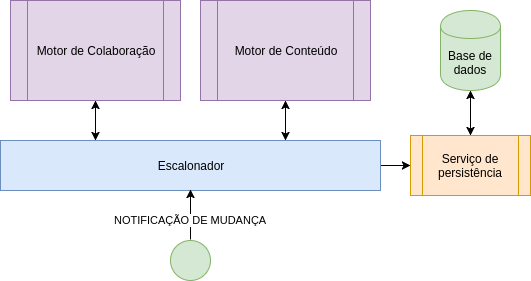
\includegraphics[scale=0.8]{images/scheduler.png}
	\end{center}
	\hspace{5.5cm}{Fonte: O Autor.}
\end{figure}

Analisando a figura \ref{scheduler}, nota-se que o escalonador é a base que sustenta a comunicação entre o serviço de persistência e os motores de recomendação, além de transformar as notificações de mudança do estado dos dados em requisições paralelas para treinamento dos itens e usuários.

Além disso, a estratégia para fusão das recomendações pode ser descrita da seguinte forma: o escalonador requisita aos \textbf{\textit{workers}} que iniciem o processo de treinamento para ambos os motores de recomendação. Ao término de ambos, o escalonador analisa as recomendações retornadas para cada item, caso seja um treinamento de toda a base de dados, ou as recomendações do item em questão, caso seja o treinamento da mudança de um item em específico, fundindo-as em uma lista única. Após a fusão de recomendações, o escalonador remove as repetições e, posteriormente, persiste as $k$ recomendações com maior nível de similaridade no banco de dados.

Por fim basta a interface de comunicação, em um momento futuro onde o usuário da API requisita recomendações, notificar o serviço de persistência para que o mesmo requisite a lista de itens similares ao usuário/item em questão (\textbf{\textit{similar}}), sem a necessidade de um processamento em tempo real, uma vez que as recomendações já foram persistidas anteriormente.

\subsection{Motor de Conteúdo} \label{motor:conteudo}

Conforme abordado na seção \nameref{recs:content_based}, os sistemas de recomendação baseados em conteúdo analisam o conteúdo de itens previamente avaliados pelo usuário. Esta seção aborda a implementação deste tipo de sistema recomendador no contexto da aplicação, dissecando os princiais tópicos relacionados a sistemas baseados em conteúdo e como foram implementados de modo a serem personalizados através dos metadados.

Para que seja possível fornecer recomendações de itens baseando-se em seu conteúdo de forma dinâmica, assim que o motor de recomendações é notificado de uma mudança relevante no estado dos dados, como apresentado na seção \nameref{motor:async}, uma série de passos são executados. Este processo pós-notificação pode ser divido em cinco partes:

\begin{enumerate}
	\item \textbf{Obtenção das informações}: carrega uma lista de todos os itens com os atributos a serem processados (\textbf{\textit{recommendable}}) declarados nos metadados.

	\item \textbf{Cálculo da similaridade}: para cada item $I_{m}$ obtido, gera uma matriz de $[m, n]$ itens com o grau de similaridade entre o item corrente e os demais.

	\item \textbf{Cálculo da proximidade}: para cada item $I_n$ da matriz de similaridades, calcula a distância de coseno entre o item $I_n$ e cada item da lista $\lbrace S_{0}$, ..., $S_{j} \rbrace$, sendo $S$ um item similar a $I_{n}$.

	\item \textbf{Persistência por proximidade}: ordena a lista de distâncias, resultante de cada item $I_{n}$, da menor distância para a maior, persistindo um ranking dos cinquenta itens mais próximos como similares do item $I_{n}$ na base de dados.

	\item \textbf{Obtenção das recomendações}: consulta a base de dados para obter os $k$ itens da lista de similares para o item $I_{n}$ e os retorna ao usuário da API.
\end{enumerate}

Como resultado final do processamento feito pelo \textbf{motor de conteúdo}, as recomendações não são retornadas ao usuário da API, mas sim persistidas no banco de dados. Isso ocorre pois o tempo de retorno se tornaria muito alto, devido a quantidade de processos a serem feitos, além do principal fato de que as notificações de mudança são recebidas pelo motor em momentos diferentes das requisições de recomendação do usuário da API. O processo de geração das recomendações, abstraído da interação com o escalonador, pode ser visto na figura \ref{content_engine}. 

\begin{figure}[h!tp]
	\caption{\label{content_engine}Funcionamento do motor de conteúdo.}
	\begin{center}
		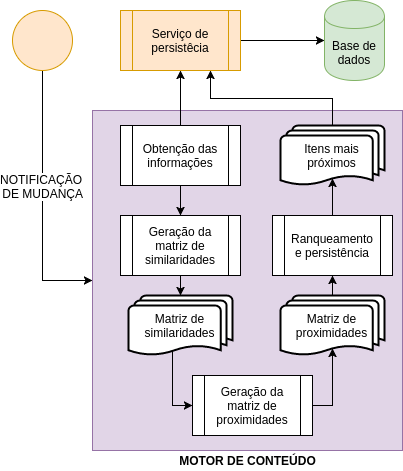
\includegraphics[scale=0.8]{images/content_engine.png}
	\end{center}
	\hspace{5.5cm}{Fonte: O Autor.}
\end{figure}

Sendo assim, o processo do motor de conteúdo pode ser definido da seguinte maneira: primeiramente o motor de conteúdo recebe uma requisição do escalonador para gerar novas recomendações ao item, devido a um novo item inserido na base ou uma alteração nas informações do mesmo. Uma vez notificada a mudança, o motor requisita ao serviço de persitência a \textbf{obtenção das informações recomendáveis}.

Para satisfazer as necessidades do motor de recomendações, o serviço de persistência de itens requisita aos metadados quais são os \textbf{atributos recomendáveis vigentes} e, a partir destes, obtém os dados decorrentes do banco de dados. Uma vez em posse destes dados, entrega-os em forma de lista.

Assim que o motor de conteúdo obtém a lista de itens, os mesmos são percorridos um a um, calculando o nível de similaridade do item em questão em contraste com os demais. O nível de similaridade é calculado através do algoritmo \textbf{TF-IDF}, abordado por \citeonline{pazzani2007content} e \citeonline{leskovec2014mining}. Este algoritmo calcula a \textbf{frequência do termo–inverso da frequência nos documentos}, ideal neste caso para transformar campos textuais em pesos numéricos, multiplicados posteriormente pelo peso de cada atributo recomendável nos metadados, gerando finalmente o grau de similaridade.

Por fim, de posse da matriz de similaridades, o motor de conteúdo percorre a mesma, item a item, calculando o grau de distância entre o item em questão e os demais itens da lista. A distância é calculada através do algoritmo da \textbf{similaridade de coseno}, que mede o espaço produto do coseno aplicado as similaridades. Após o processamento, os $k$ itens de menor distância são persistidos no banco de dados pelo serviço de persistência de itens, que atribui a \textit{tag} \textbf{\textit{similar}} a lista de itens persistidos.

\subsection{Motor Colaborativo} \label{motor:colaborativo}

Assim como o motor de conteúdo, o motor colaborativo opera sobre matrizes, com exceção de que, ao invés de matrizes que contrastam itens, o motor gera matrizes que contrastam usuários e itens. Para isso, são necessários registros que relacionem usuários e itens a um peso dado, as avaliações. Estas avaliações podem ser binárias (\textit{like}/\textit{unlike}) ou enumeradas, como avaliações de zero a cinco estrelas, por exemplo.

Recomendações utilizando o método colaborativo, como apresentadas na seção \nameref{recs:collaborative_based}, podem ser orientadas a usuário ou a item. Como forma de compensar o motor de conteúdo, que se baseia inteiramente em itens, o método empregado neste motor será orientado a usuário. Sendo assim, o método de recomendação colaborativa orientado a usuário implementado nesta aplicação pode ser dividido em seis partes:

\begin{enumerate}
	\item \textbf{Obtenção das avaliações}: O motor colaborativo requisita ao serviço de persistência os registros válidos de recomendações de usuários a itens.

	\item \textbf{Construção da matriz de intersecções}: para acada usuário $U_{n}$, identifica as intersecções, ou seja, itens avaliados por ambos os usuários em questão, gerando uma matriz de intersecções.

	\item \textbf{Construção da matriz de similaridades}: a partir da matriz de intersecções, para cada usuário $U_{n}$ calcula a \textbf{correlação de pearson} entre o usuário $U_{n}$ e os usuários $\lbrace S_{0}$, ..., $S_{j} \rbrace$ pertencentes a lista de intersecções, utilizando como base as avaliações de ambos sobre o item.

	\item \textbf{Cálculo da distância}: após a construção da matriz de similaridades, para cada usuário $U_{n}$ pertencente a matriz, calcula a \textbf{distância euclidiana} entre o usuário $U_{n}$ e os usuários $\lbrace S_{0}$, ..., $S_{j} \rbrace$ considerados similares na matriz, gerando uma matriz de usuários mais próximos.

	\item \textbf{Persistência por proximidade}: para cada usuário $U_{n}$ da matriz de proximidade, persiste os itens dos $k$ usuários mais próximos no banco de dados como recomendações ao usuário em questão.

	\item \textbf{Obtenção das recomendações}: consulta a base de dados para obter os $k$ itens da lista de similares para o usuário $U_{n}$ e os retorna ao usuário da API.
\end{enumerate}

A medida que o número de avaliações aumenta, em corelação com o tempo de vida da aplicação, as recomendações do motor de colaraboração tendem a ser mais precisas, uma vez que fazem uso da própria manifestação dos usuários para definir as similaridades. A interação do motor colaborativo com o resto da aplicação pode ser visto na figura \ref{collaborative_engine}.

\begin{figure}[h!tp]
	\caption{\label{collaborative_engine}Funcionamento do motor colaborativo.}
	\begin{center}
		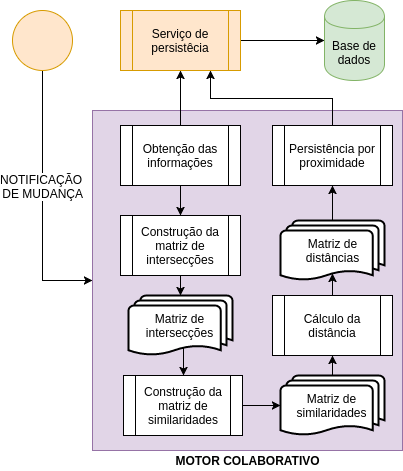
\includegraphics[scale=0.8]{images/collaborative_engine.png}
	\end{center}
	\hspace{5.5cm}{Fonte: O Autor.}
\end{figure}

Analisando a figura \ref{collaborative_engine}, nota-se que o fluxo de funcionamento do motor colaborativo se assemelha muito ao motor de conteúdo. O ponto de diferença está no conteúdo das matrizes, onde no motor de conteúdo são preenchidas com itens e suas similaridades, já no motor colaborativo são preenchidas com as intersecções de avaliações de usuários e, posteriormente, com a similaridade entre eles.

\section{Testes e Implementação} \label{testes}

Durante o processo de desenvolvimento do protótipo desta aplicação, foi necessária a utilização de um grupo de dados de teste não só nos padrões especificados pela API, mas também coerente com sua semântica de relações. Dessa forma, os testes do funcionamento das recomendações foram executados com a utilização de uma base real de usuários, itens e avaliações, contendo um volume de dados suficiente para que os objetivos deste trabalho fossem assegurados.

A base de dados em questão é a do projeto \textbf{MovieLens}, proposto por \citeonline{harper2016movielens}, comumente utilizada para aplicações com este fim devido ao fato de possuir inúmeras opções de tamanhos diferentes, preenchidas com dados retirados de ambientes de produção. Além disso, a base de testes acima descrita, foi amplamente utilizada para testar a assertividade de algoritmos durante o \textbf{NetflixPrize}, evento promovido pela empresa \textbf{Netflix} para eleger os algoritmos de recomendações mais assertivos \cite{bennett2007netflix}.

Acerca dos testes e implementações efetuadas, esta seção disseca tal processo em quatro partes. Primeiro são apresentadas as implementações referentes ao preenchimento do conjunto teste de dados e seus resultados. Logo após, é apresentado o processo de documentação automática, implementado visando a contribuição da comunidade. Em seguida, é apresentada a composição de cada um dos \textit{scripts} que efetuam a instalação da API e sua inicalização, além da atualização de eventuais dependências do projeto. Por fim, são abordadas, de forma mais específica, as tecnologias utilizadas durante o desenvolvimento desta aplicação.

\subsection{\textit{Seed} de Dados} \label{seed}

Como forma de automatizar o processo de geração dos dados de teste da aplicação, foi implementado um \textit{script}, podendo ser chamado pelo usuário da API, com a função de fazer o \textit{download} do conjunto de dados do projeto \textbf{MovieLens}, configurar os metadados correspondentes e fazer a persistência das informações. Este \textit{script}, executado pela linha de comando do sistema operacional e intitulado \textbf{seed.sh}, visa facilitar o processo de primeira inicialização da aplicação, atraindo novos usuários e aumentando o número de colaboradores no projeto.

Além disso, o \textit{seed} de dados proporciona um teste, quase que imediato, do funcionamento completo da API. Ao passo que o \textit{script} finaliza sua execução, o usuário da API já pode fazer requisições de recomendações, visualizando de forma simples e concisa o potencial da mesma. O processo de \textit{seed} de dados pode ser dividido em quatro passos:

\begin{enumerate}
	\item \textbf{\textit{Download} do conjunto de dados}: o \textit{script} executa o \textit{download} do conjunto de dados com aproximadamente um milhão de registros (itens, usuários e avaliações).

	\item \textbf{Conversão dos dados para o padrão da API}: a classe conversora do \textit{seeder} de dados converte o padrão recebido pelo padrão utilizado na API (JSON).

	\item \textbf{Persistência dos dados}: após a conversão , a classe conversora invoca o serviço de persistência para persistir toda o conjunto de dados de uma só vez.

	\item \textbf{Configuração dos metadados e treinamento da base}: a classe conversora configura os primeiros metadados de acordo com o padrão recebido e os persiste na base através do serviço de persistência. Ao ser notificado da alteração no estado da base, o motor de recomendações treina o conjunto recebido.
\end{enumerate}

Caso o usuário da API queira preencher a aplicação com seus próprios dados, o mesmo deve executar o \textit{script} de inicalização, fazendo com que os dados de exemplo sejam removidos e as configurações redefinidas. O processo de inicialização da API e as configurações são abordadas na seção \nameref{init}.

\subsection{Instalação e Inicialização} \label{init}

Além da automatização na criação de dados de exemplo, apresentada na seção \nameref{seed}, foram implementados outros \textit{scripts} auxiliares de instalação, inicalização e atualização de dependências, nomeados \textbf{setup.sh}, \textbf{start.sh} e \textbf{update\_dependencies.sh} respectivamente. Todos estres \textit{scripts}, contidos na pasta \textit{"scripts"} da aplicação, visam aumentar a simplicidade no uso da API e, consequentemente possibilitar a utilização pela comunidade em geral.

O \textit{script} de instalação (\textbf{setup.sh}) tem como função instalar todas as dependências iniciais do projeto, além de configurar completamente o ambiente virtual no qual a aplicação é executada. Este ambiente virtual serve para que o escopo das dependências e dos pacotes instalados pelo \textit{script} de instalação não poluam a máquina do usuário da API.

Além disso, o \textit{script} de inicialização requisita algumas informações necessárias para a configuração inicial da aplicação, tais como o nome, usuário e senha do banco de dados e a palavra secreta utilizada na autenticação. Estas configurações guiam o funcionamento da API como um todo e podem ser modificados a qualquer momento no arquivo de variáveis de ambiente (\textbf{env.py}).

O \textit{script} de inicalização (\textbf{start.sh}) tem como função inicializar o serviço \textit{web} da aplicação, ativando o ambiente virtual criado pelo \textit{script} de instalação e executando o arquivo que inicializa a API. Assim que iniciada, a aplicação é acessível através de um endereço IP e porta específicos, configuráveis através do arquivo de variáveis de ambiente (\textbf{env.py}).

Em caso de adição ou modificação na versão de alguma das dependências da aplicação, o \textit{script} \textbf{update\_dependencies.sh} tem como objetivo atualizar as dependências já listadas anteriormente, além de instalar novas dependências recém adicionadas. As dependências do projeto podem ser adicionadas no arquivo de requerimentos da aplicação (\textbf{requirements.txt}).

\subsection{Documentação}

Durante boa parte do processo de desenvolvimento da aplicação, foi implementada a documentação dos módulos, funções e métodos escritos, visando facilitar a manutenção futura da aplicação e a contribuição da comunidade. Tais trechos de código documentados são dinamicamente carregados em uma documentação automática, gerada a partir de um \textit{template} que converte os comentários acima do código, os parâmetros de entrada e os tipos de retorno para itens da documentação. Um exemplo de página gerada pela documentação pode ser visto na figura \ref{docs}.

\begin{figure}[h!tp]
	\caption{\label{docs}Documentação automática da API.}
	\begin{center}
		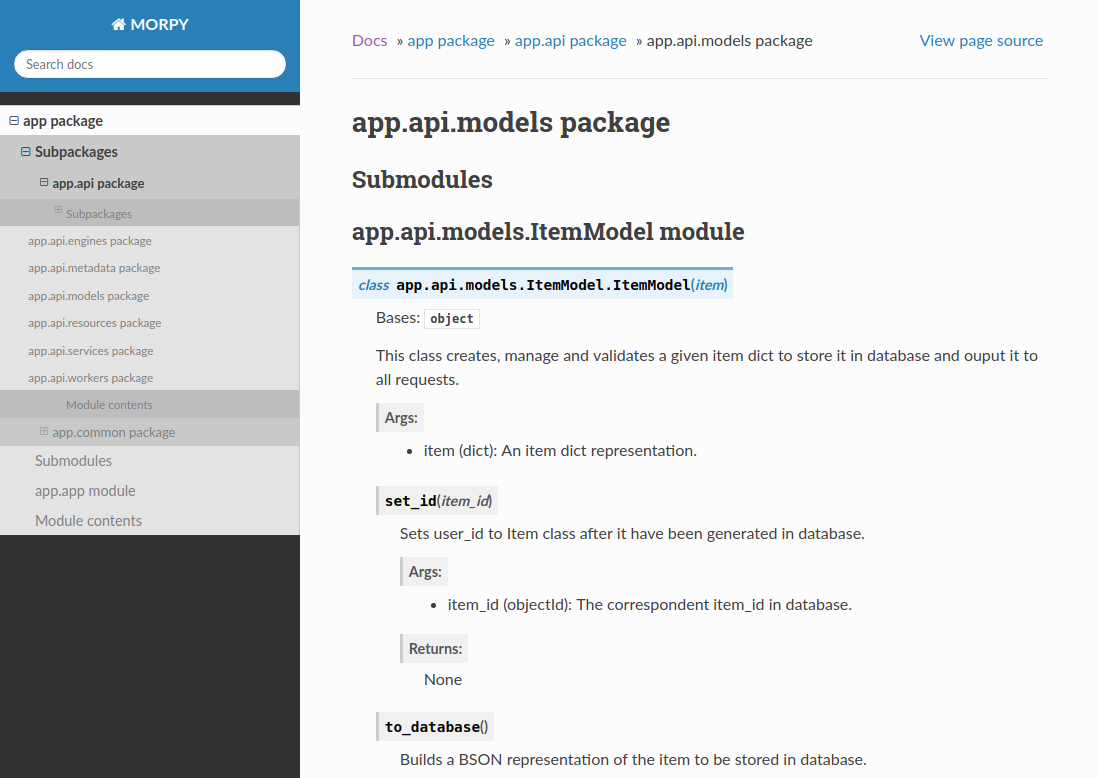
\includegraphics[scale=0.55]{images/docs.png}
	\end{center}
	\hspace{5.5cm}{Fonte: O Autor.}
\end{figure}

A documentação conta com toda a hierarquia correspondente a estrutura da API, deixando visível ao usuário a estrutura empregada e a localização de cada classe e módulo implementados. Além disso, cada módulo documentado possui uma breve descrição das suas funcionalidades. Nas classes de cada módulo são especificados os parâmetros de entrada de cada método, além do tipo de dado esperado e uma descrição do retorno. Se preferir, o usuário pode utilizar um campo de pesquisa para encontrar o método ou módulo desejado.

\subsection{Tecnologias Utilizadas} \label{tecnologias}

Para tornar possível a implementação desta aplicação em tempo hábil, foram empregadas várias tecnologias, escolhidas de modo a fomentar a utilização pela comunidade atual de desenolvedores e a iniciativa \textit{open-source}. O quadro \ref{technologies} apresenta as principais tecnologias utilizadas para a execução deste trabalho e a suas respectivas categorias.

\begin{quadro}[htp]

	\caption{\label{technologies}Tecnologias utilizadas durante a implementação.}

	\begin{center}
	\begin{tabular}{|l|l|}
	\hline
	\textbf{Categoria} 			& \textbf{Tecnologia}   \\ \hline
	Sistema operacional 		& Linux Ubuntu LTS      \\ \hline
	Banco de dados 		   		& MongoDB  				\\ \hline
	Linguagens de programação   & Python e Shell script \\ \hline
	Controle de versão          & Github   				\\ \hline
	Framework de API        	& Flask      			\\ \hline
	Framework de persistência 	& PyMongo 				\\ \hline
	Gerenciador de dependências & Conda 				\\ \hline
	Ferramenta de testes		& Postman				\\ \hline
	Documentação automática		& Sphinx				\\ \hline
	\end{tabular}
	\end{center}

	\hspace{3.2cm} {\fontsize{10pt}{\baselineskip}\selectfont Fonte: O autor.}

\end{quadro}

Visando maximizar a legibilidade e a simplicidade do código fonte, foi utilizada a linguagem \textbf{Python} como base para toda a aplicação. Além disso, a escolha da linguagem Python também se dá pelo fato de existirem módulos de \textit{machine learning} amplamente utilizados em aplicações deste gênero pela comunidade de desenvolvedores Python. Entre eles o \textbf{SciKit}, proposto por \citeonline{pedregosa2011scikit} e utilizado nesta aplicação, equilibrando de forma eficiente o desempenho e a abstração de certos processos.

Como forma de complementar a escolha de legibilidade e desempenho através da linguagem Python, o banco de dados utilizado pela aplicação é o \textbf{MongoDB}. Tal banco de dados foi escolhido devido a sua escalabilidade com grandes volumes de dados e seu tempo de consulta superior aos bancos relacionais. Além disso, a orientação a documentos BSON, inspirados no padrão JSON, facilitaram e muito a comunicação entre banco de dados e aplicação \cite{chodorow2013mongodb}.

Os \textit{scripts} utilizados para automatização, apresentados da seção \nameref{init}, foram escritos na linguagem \textbf{Shell Script}, tendo sua execução pelo \textit{shell} do sistema operacional \textbf{Linux Ubuntu}. Por hora, estes \textit{scripts} apenas são suportados por este sistema operacional e seus derivados.

Para armazenamento e controle de versão do código foi utilizado o \textbf{Github}, ferramenta aberta e colaborativa de repositórios de versão, comumente utilizada pela comunidade. Além do controle de versão, a ferramenta permite que outros desenvolvedores ramifiquem esta aplicações a sua maneira, disseminando a utilização desta API, um dos objetivos deste trabalho \cite{dabbish2012social}.

É importante ressaltar que todas as ferramentas utilizadas durante a execução deste trabalho são de código aberto/livre, escolhidas para fomentar a utilização da aplicação, através de ferramentas já conhecidas e amplamente utilizadas pela comunidade, tais como \textbf{Github}, \textbf{Python}, \textbf{MongoDB}, etc.